\chapter{Simulation}
\label{ch:simulation} 
Since a real copter was not available for testing, 2 proof-of-concept simulation were performed. In the first one the controller has been used with an extended Kalman filter but no sensor has been used: the state of the copter is estimated by mean of the control signal and the model of the copter; the second simulation demonstrates the feasibility of a full Kalman filter update and predict behavior: an real AHRS sensor is used to update the state of the copter accordingly to the sensors data and a constant control signal.

\section{Kalman filter in predict-only mode}

The node core functionality is implemented in the extended Kalman filter and in the controller, a layout of the node is depicted in \autoref{fig:node040}. The set-point of the copter is computed by the node on the basis of 10 primitives that can be called via a tool that acts as remote controller for the copter, the communication between the node and the controller is realized via a TCP connection.\\
The controller block \texttt{ctrl} reads the copter state from the block \texttt{state} and the set-point from the block \texttt{setpoint} , than computes and store the control action in \texttt{ctrl\_action}. The Kalman filter block \texttt{kf\_pred\_cptr} in turns reads the state and the control action applied and write the estimate of the state back.

Other blocks are however necessary:
\begin{itemize}
	\item \texttt{ptrig1} is the i-block in charge to call all the c-block of the node (except the graphic dump) in an infinite loop with a period of 1ms;
	\item \texttt{tgj\_gen} is a c-block responsible for generating the current set-point: it receives the trajectory primitive from a tcp connection and computes the actual copter set-point as a function of the time;
	\item \texttt{state} is a i-block that store the state of the copter in virtual memory;
	\item \texttt{setpoint} is a i-block that store the set-point of the copter in virtual memory;
	\item \texttt{ctrl\_action} is a i-block that store the current applied control action in virtual memory;
	\item \texttt{timing} generates a virtual clock allowing to simulate the system beyond the actual computation capabilities of the computer platform.
	\item \texttt{graphic\_dump} opens a gtk 2-D graphic interface showing the position of the copter; a screenshot is reported in \autoref{fig:gfxdump1};
	\item \texttt{ptrig\_graphic} trigs \texttt{graph\_dump} with a period of 10 ms;
\end{itemize}

The configuration file of the node is here reported:
	
	
\begin{lstlisting}[language={[5.0]Lua},]
local bd = require("blockdiagram")

return bd.system {
  imports = {
    "types/stdtypes/stdtypes.so",
    "types/control/control_types.so",
    "blocks/ptrig/ptrig.so",
    "blocks/control/shm.so",
    "blocks/control/dump_ctrl.so",
    "blocks/copter/ctrl_copter.so",
    "blocks/copter/prim_trj_gen.so",
    "blocks/copter/kf_predict_copter.so",
    "blocks/control/dump_state.so",
    "blocks/copter/copter_graphic_dump.so",
    "blocks/control/dump_time_stat.so",
    "blocks/webif/webif.so",
  },

  blocks = {
    { name = "ptrig1" , type = "std_triggers/ptrig" },
    { name = "ptrig_graphic", type = "std_triggers/ptrig" },
    { name = "ctrl_action"  , type = "control/shm" },
    { name = "state"  , type = "control/shm" },
    { name = "setpoint"  , type = "control/shm" },
    { name = "ctrl" , type = "copter/ctrl_copter" },
    { name = "ctrl_dump" , type = "control/dump_ctrl" },
    { name = "state_dump" , type = "control/dump_state" },
    { name = "kf_pred_cptr" , type = "copter/kf_predict_copter" },
    { name = "tgj_gen" , type = "copter/prim_trj_gen" },
    { name = "graph_dump"  , type = "copter/copter_graphic_dump"    },
    { name = "timing"  , type = "control/dump_time_stat"    },
    { name = "webif1"  , type = "webif/webif"    },
  },

  connections = {
    { src="ctrl.ctrl_action" , tgt="ctrl_action" },
    { src="ctrl.ctrl_action" , tgt="ctrl_dump" },
    { src="state" , tgt="ctrl.state" },
    { src="setpoint" , tgt="ctrl.setpoint" },
    { src="kf_pred_cptr.stt_out" , tgt="state" },
    { src="kf_pred_cptr.stt_out" , tgt="state_dump" },
    { src="state" , tgt="kf_pred_cptr.stt_in"  },
    { src="ctrl_action" , tgt="kf_pred_cptr.ctrl_in" },
    { src="tgj_gen.setpoint_out"  , tgt="setpoint" },
    { src="state" , tgt="tgj_gen.state_in" },
    { src="state"      , tgt="graph_dump.state"  },
    { src="setpoint"    , tgt="graph_dump.setpoint"  },
  },

  configurations = {
    {
      name="webif1",
      config = { port="8888" },
    },
		{
			name="kf_pred_cptr" ,
			config = {
				mass		= 1 	,
				J_xx		= 0.01,
				J_yy		= 0.01,
				J_zz		= 0.01,
				dt		= 0.001	,
				process_noise	= 0	,
			},
		},
		{
			name="ctrl_action" ,
			config = {
				shm_name="/ctrl_action" ,
				type_name="struct ControlAction",
			},
		},
		{
			name="setpoint" ,
			config = {
				shm_name="/setpoint" ,
				type_name="struct SetPoint",
			},
		},
		{
			name="state" ,
			config = {
				shm_name="/state" ,
				type_name="struct State",
			},
		},
		{
			name="tgj_gen" ,
			config = {
				dt	= 0.001	;
				zmq_address = "tcp://127.0.0.1:8890"
			},
		},
		{
			name="ctrl" ,
			config = {
				mass		= 1	,
				inertia_xx	= 0.01,
				inertia_yy	= 0.01,
				inertia_zz	= 0.01,
				k1		= 1	,--0.9	,
				l1		= 5	,--5	,	-- i.e. max speed for static set-point
				k2		= 10	,--8	,
				l2		= 10	,--8	,
				kp		= 100	,
				kd		= 10	,
				hysteresis_thr	= 0.01	,
				max_thrust	= 20	,
				max_torque_xx	= 3	,
				max_torque_yy	= 3	,
				max_torque_zz	= 3	,
			},
		},
		{
			name="timing" ,
			config = {
				period		= 60*1000	;
				update_rate	= 0.001		;
			},
		},
		{
			name="ptrig1" ,
			config = {
				period = {sec=0, usec=1000 },
				trig_blocks={
					{ b="#ctrl"		, num_steps=1, measure=0 },
					{ b="#kf_pred_cptr"	, num_steps=1, measure=0 },
					{ b="#tgj_gen"		, num_steps=1, measure=0 },
					{ b="#timing"		, num_steps=1, measure=0 },
				},
			},
		},
		{
			name="graph_dump" ,
			config = {
				zoom = 5 ;
				max_q = 2 ;
			},
		},
		{
			name="ptrig_graphic" ,
			config = {
				period = {sec=0, usec=10000 },
				trig_blocks={
					{ b="#graph_dump"	, num_steps=1, measure=0 },
        },
      },
    },
  },
}
\end{lstlisting}
\subsection{Launching the node}
The node can be lunched by calling the script\\
\texttt{ubx-control/test/04-working\_ctrl/launch.sh}\\
This script also executes the gtk app \texttt{fake\_planner} specifying with an argument to connect to \texttt{tcp://127.0.0.1:8890} (obviusly the node is configured to listen at the same TCP address and port).
\graffito{The name of the remote controller executable is \texttt{fake\_planner} because there may be an actual \emph{mission} planner (or supervisor) controlling the drone instead of a human operator.}
Then the script launches and deploys the node. Messages from the node are dumped to the terminal but the state of the node can be also checked via a web interface at \texttt{http://127.0.0.1:8888}.

\newpage
\begin{figure}
	\centering
	\frame{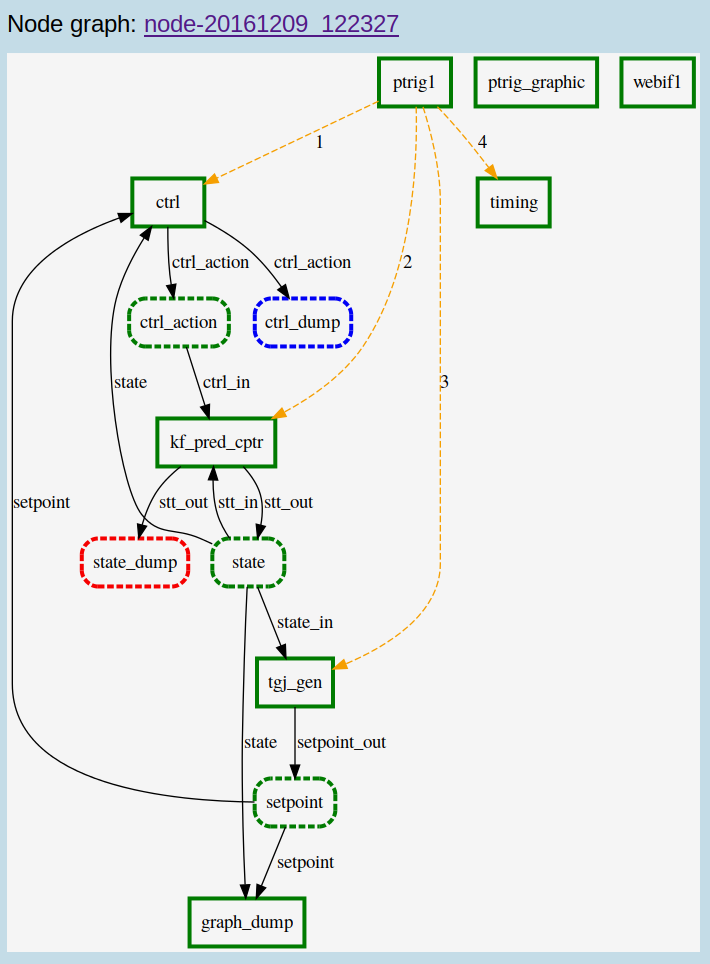
\includegraphics[width=1\textwidth]{node04}}
	\caption{The node used for the simulation in predict-only mode}
	\label{fig:node040}
\end{figure}
\clearpage

\newpage
\begin{figure}
	\centering
	\frame{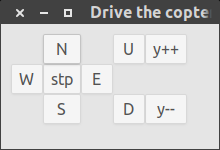
\includegraphics[width=0.3\textwidth]{fakeplanner}}
	\frame{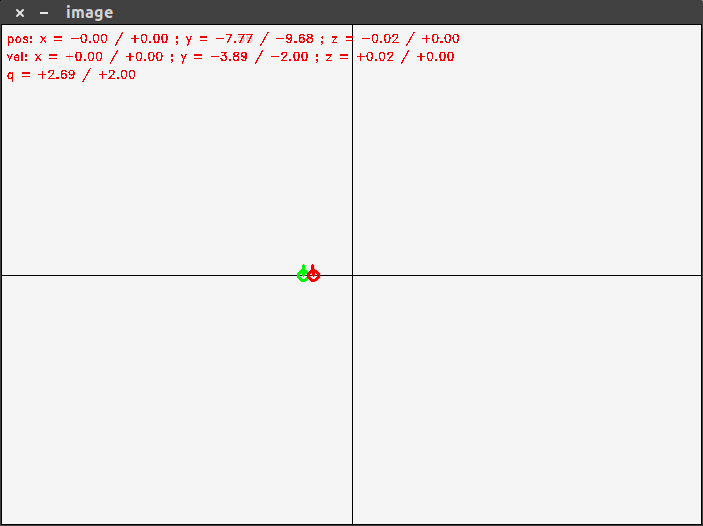
\includegraphics[width=0.8\textwidth]{gfxdump1}}
	\caption{The remote controller HMI interface and the graphic dump of the copter state and set-point}
	\label{fig:gfxdump1}
\end{figure}
\clearpage


\section{Kalman filter in update mode}
The second simulation was performed in a configuration where the Kalman filter is used to update the estimate of the state of the vehicle by reading from an attitude and heading reference system (AHRS) \autocite{bib:wikiahrs}. This application is a proof-of-concept demonstration for sensor fusion and the controller has no role here, the control action is constant (i.e. no feedback) and manually tuned to make the copter hover. The Kalman filter then update the copter attitude with the data from the sensors and accordingly predict the estimate of the position too.\\
The AHRS used is a USB device from Hardkernel \autocite{bib:ahrsproduct}; it embeds a triple axis gyroscope, a triple axis accelerometer and a triple axis magnetometer, plus it embeds an extended Kalman filter (so data if pre-filtered and pre-fused); data can be read via a I2C or UART or USB serial interface. The i-block used to read is a bridge written in C++ named \texttt{sensor\_myAHRS} and can be found in the \texttt{ubx-control} project.

The node can be launched by executing:
\begin{lstlisting}[language=bash]
cd ubx-control/test/06_test_myAHRS/
ubx_launch -c 06.usc -d deploy.udc
\end{lstlisting}

As expected, if the AHRS is horizontal the Kalman filter will just correct the heading: since the AHRS embeds a magnetometer, the filter has been told to map the $x$ axis of the fixed reference frame the copter is moving in to the magnetic North.\\
If the AHRS is oriented, the copter will orient accordingly and will start moving around. Note that however the copter will loose elevation, since the controller generates no torque and just the thrust exactly sufficient to hover horizontally.\\

As in the previous simulation, it follows the configuration of the node:

\begin{lstlisting}[language={[5.0]Lua},]
local bd = require("blockdiagram")

return bd.system {
  imports = {
    "types/stdtypes/stdtypes.so",
    "types/control/control_types.so",
    "blocks/ptrig/ptrig.so",
    "blocks/webif/webif.so",
    "blocks/control/shm.so",
    "blocks/control/dump_ctrl.so",
    --"blocks/copter/ctrl_copter.so",
    "blocks/copter/prim_trj_gen.so",
    "blocks/copter/kf_predict_copter.so",
    "blocks/control/dump_state.so",
    "blocks/copter/copter_graphic_dump.so",
    "blocks/control/dump_time_stat.so",
    "blocks/control/sensor_myAHRS.so",
    "blocks/control/fake_ctrl.so",
    "blocks/control/kf_update.so",
  },

  blocks = {
    { name = "ptrig1"	, type = "std_triggers/ptrig"		},
    { name = "webif1"	, type = "webif/webif"				},
    { name = "ptrig_graphic", type = "std_triggers/ptrig"	},
	{ name = "ctrl_action"	, type = "control/shm"			},
	{ name = "state"	, type = "control/shm"				},
	{ name = "setpoint"	, type = "control/shm"				},
	{ name = "ctrl"		, type = "control/fake_ctrl"		},
	{ name = "ctrl_dump"	, type = "control/dump_ctrl"			},
	{ name = "state_dump"	, type = "control/dump_state"			},
	{ name = "kf_pred_cptr"	, type = "copter/kf_predict_copter"		},
	{ name = "tgj_gen"	, type = "copter/prim_trj_gen"				},
	{ name = "graph_dump"	, type = "copter/copter_graphic_dump"	},
	{ name = "timing"	, type = "control/dump_time_stat"		},
	{ name = "ahrs"       , type = "control/sensor_myAHRS"    	},
	{ name = "kf_upd"       , type = "control/kf_update"    	},
  },

  connections = {
	{ src="ctrl.control_out"	, tgt="ctrl_action"			},
	{ src="ctrl.control_out" 	, tgt="ctrl_dump"			},
	{ src="kf_pred_cptr.stt_out"	, tgt="state"			},
	{ src="kf_pred_cptr.stt_out"	, tgt="state_dump"		},
	{ src="state"			, tgt="kf_pred_cptr.stt_in"		},
	{ src="ctrl_action"		, tgt="kf_pred_cptr.ctrl_in"	},
	{ src="tgj_gen.setpoint_out"	, tgt="setpoint"		},
	{ src="state"			,tgt="tgj_gen.state_in"			},
	{ src="state"			, tgt="graph_dump.state"		},
	{ src="setpoint"		, tgt="graph_dump.setpoint"		},
	{ src="kf_upd.state_out"        , tgt="state_dump"              },
	{ src="kf_upd.state_out"        , tgt="state"                   },
	{ src="state"                   , tgt="kf_upd.state_in"         },
	{ src="ahrs"                     , tgt="kf_upd.sensor_in"       },
  },
  
  configurations = {
	{
		name="webif1",
		config = { port="8888" },
	},
	{
		name="kf_pred_cptr" ,
		config = {
			mass		= 1 	,
			J_xx		= 0.01,
			J_yy		= 0.01,
			J_zz		= 0.01,
			dt		= 0.001	,
			process_noise	= 0.01	,
		},
	},
  {
	name="ctrl_action" ,
	config = {
		shm_name="/ctrl_action" ,
		type_name="struct ControlAction",
    },
  },
  {
    name="setpoint" ,
    config = {
      shm_name="/setpoint" ,
      type_name="struct SetPoint",
    },
  },
  {
    name="state" ,
    config = {
      shm_name="/state" ,
      type_name="struct State",
    },
  },
  {
    name="tgj_gen" ,
    config = {
      dt	= 0.001	;
    },
  },
  {
    name="ctrl" ,
    config = {
      filepath_U="U",
    },
  },
  {
    name="ahrs",
    config = {
      device_path = "/dev/ttyACM0"	,
      quaternion_cov = 0.0001		,
    }
  },
  {
    name="kf_upd" ,
    config = {
      filepath_H	= "H"	,
    },
  },
  {
    name="timing" ,
    config = {
      period		= 60*1000	,
      update_rate	= 0.001		,
    },
  },
  {
          name="ptrig1" ,
          config = {
            period = {sec=0, usec=1000 },
            trig_blocks={
            { b="#ctrl"		, num_steps=1, measure=0 },
            { b="#kf_upd"		, num_steps=1, measure=0 },
            { b="#kf_pred_cptr"	, num_steps=1, measure=0 },
            { b="#tgj_gen"		, num_steps=1, measure=0 },
            { b="#timing"		, num_steps=1, measure=0 },
          },
        },

      },
      {
        name="graph_dump" ,
        config = {
        zoom = 5 ;
        max_q = 2 ;
      },

    },
    {
      name="ptrig_graphic" ,
      config = {
        period = {sec=0, usec=1000 },
        trig_blocks={
          { b="#graph_dump"	, num_steps=1, measure=0 },
        },
      },
    },
  },
}
\end{lstlisting}

\newpage
\begin{figure}
	\centering
	\frame{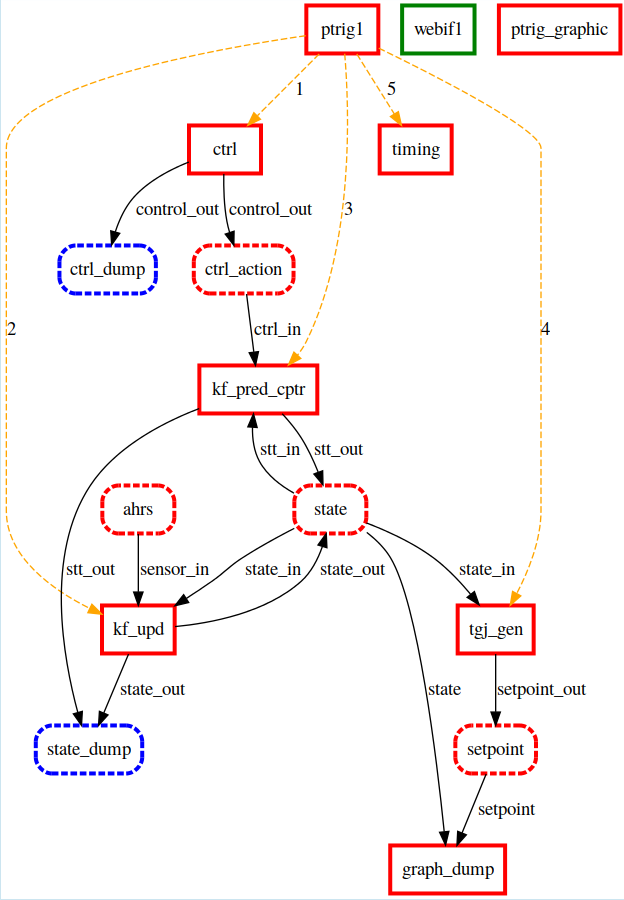
\includegraphics[width=1\textwidth]{node06}}
	\caption{The node used for the simulation in update mode}
	\label{fig:node060}
\end{figure}
\clearpage